\documentclass[11pt]{article}

\usepackage[margin=1in]{geometry}
\usepackage{amsmath,amssymb,amsthm,mathtools}
\usepackage[authoryear,round]{natbib}
\usepackage{enumitem}
\usepackage{xcolor}
\usepackage{tikz}
\usetikzlibrary{arrows.meta,positioning}
\usepackage[colorlinks=true,linkcolor=blue!50!black,citecolor=blue!50!black,urlcolor=blue!50!black]{hyperref}

\newtheorem{proposition}{Proposition}[section]
\newtheorem{example}[proposition]{Example}
\newtheorem{remark}[proposition]{Remark}
\newtheorem{definition}[proposition]{Definition}

\newcommand{\dd}[2]{\frac{\partial #1}{\partial #2}}
\newcommand{\R}{\mathbb{R}}

\title{Why the Initial-Value Problem Makes No Sense for the Hamilton--Jacobi Equation}
\author{}
\date{}

\begin{document}

\maketitle

\begin{abstract}
\noindent
Hamilton's canonical equations $\dot q=\partial H/\partial p$, $\dot p=-\partial H/\partial q$ admit a genuine initial-value problem: fix $(q_0,p_0)\in T^*Q$ at a time $t_0$ and the future is determined, by the ordinary Picard--Lindel\"of theorem. The Hamilton--Jacobi equation $\partial S/\partial t + H(q,\partial S/\partial q,t)=0$ is often introduced as though it carried an analogous initial-value problem, and it is tempting---since the equation is first order in $t$---to imagine that fixing $S$, or $S$ together with $\partial S/\partial q$, at a single point $(q_0,t_0)$ should play the same role for the field $S(q,t)$ that fixing $(q_0,p_0)$ plays for a single trajectory. This is false, and provably so. We exhibit an explicit pair of solutions of the free-particle Hamilton--Jacobi equation that agree in value and gradient at one spacetime point but disagree everywhere else, showing that pointwise data of this kind pins down nothing beyond that single point. We then identify the structural reason: the characteristics of the Hamilton--Jacobi equation are exactly Hamilton's canonical equations, so a single dynamical trajectory is exactly a characteristic curve of the PDE, and the general theory of first-order PDE says that data prescribed along a characteristic is never free Cauchy data---it is either automatically consistent with the equation, and so carries no information transverse to the curve, or it is inconsistent with the equation altogether. The only notion of ``initial data'' that is well posed for the Hamilton--Jacobi equation is Cauchy data on an entire noncharacteristic hypersurface: a full function $S_0(q)$, not a point and not a curve. We close by explaining, via the correspondence between such data and Lagrangian submanifolds of $T^*Q$, why this correct notion is doing something conceptually different from---and much richer than---what Hamilton's own initial-value problem does, and why even it is only locally well posed in time.
\end{abstract}

\section{Introduction}
\label{sec:intro}

Two objects sit side by side in every treatment of classical mechanics. The first is Hamilton's canonical system,
\begin{equation}
\label{eq:Ham}
\dot q^i = \dd{H}{p_i}, \qquad \dot p_i = -\dd{H}{q^i}, \qquad i=1,\dots,n,
\end{equation}
a system of $2n$ ordinary differential equations on phase space $T^*Q$. The second is the Hamilton--Jacobi equation,
\begin{equation}
\label{eq:HJ}
\dd{S}{t} + H\Big(q,\dd{S}{q},t\Big) = 0,
\end{equation}
a single partial differential equation for a scalar function $S(q,t)$. Textbooks derive~\eqref{eq:HJ} from~\eqref{eq:Ham} (or vice versa) in a few lines, and the two are indeed equivalent in a precise sense made rigorous by Jacobi's theorem on complete integrals. That equivalence, together with the fact that~\eqref{eq:HJ} is written as ``$\partial S/\partial t$ equals something,'' first order in $t$ just as~\eqref{eq:Ham} is first order in $t$, invites a natural-seeming question: what is the initial-value problem for the Hamilton--Jacobi equation? If one can fix $(q_0,p_0)$ at $t_0$ and thereby determine the entire future of~\eqref{eq:Ham}, should one not be able to fix $S(q_0,t_0)$---perhaps together with $\partial S/\partial q$ there, so as to match the amount of data $(q_0,p_0)$ supplies---and thereby determine the entire future of~\eqref{eq:HJ}?

The answer is no, and the purpose of this paper is to explain exactly why, in enough detail that the failure is not merely asserted but demonstrated. The short version is a type mismatch. The unknown in~\eqref{eq:Ham} at a given time is a point of $T^*Q$: $2n$ real numbers. The unknown in~\eqref{eq:HJ} at a given time is a function of $q$ on all of $Q$: an element of an infinite-dimensional space. An equation that is ``first order in $t$'' for an object of the second kind does not, in general, admit initial data at a point, for exactly the same reason that no evolution equation for a field---the heat equation, the wave equation, ordinary fluid dynamics---admits initial data at a point. What is special about the Hamilton--Jacobi equation is not that this general PDE fact holds, but \emph{why} it holds in a way that is unusually easy to state precisely: the characteristics of~\eqref{eq:HJ} are exactly the trajectories of~\eqref{eq:Ham}, so the single most natural-looking candidate for ``initial data along a trajectory'' turns out to be data prescribed along a characteristic curve of the PDE---which the general theory of first-order PDE identifies as precisely the case in which prescribed data carries no genuine information at all.

Section~\ref{sec:two-objects} separates two objects that share the name ``action'' and are routinely conflated. Section~\ref{sec:ham-ivp} recalls why~\eqref{eq:Ham} has a genuine, finite-dimensional initial-value problem. Section~\ref{sec:counterexample} gives an explicit counterexample: two solutions of the same Hamilton--Jacobi equation, agreeing in value and gradient at one point, disagreeing everywhere else. Section~\ref{sec:characteristics} supplies the structural explanation, via the method of characteristics, for why this had to happen, and sharpens it to the strongest available form of the failure: data along a single trajectory is not merely insufficient, it is data on a characteristic surface, which is a degenerate case of the Cauchy problem in a precise technical sense. Section~\ref{sec:cauchy} describes the notion of initial data that \emph{does} work, and explains geometrically why it is not doing the same job as~\eqref{eq:Ham}'s initial-value problem. Section~\ref{sec:discussion} discusses why the confusion is nonetheless natural, and identifies a legitimate practice that resembles it without being it. Section~\ref{sec:conclusion} concludes.

\section{Two objects sharing one name}
\label{sec:two-objects}

Fix a Lagrangian $L(q,\dot q,t)$ and a particular solution $q(t)$ of the Euler--Lagrange equations, already known. One can attach to this single curve a number
\begin{equation}
\sigma(t) = \int_{t_0}^t L\big(q(s),\dot q(s),s\big)\, ds ,
\end{equation}
which obeys the trivial ordinary differential equation $\dot\sigma = L(q(t),\dot q(t),t)$ with $\sigma(t_0)=0$: a quadrature, nothing more, and an entirely well-posed initial-value problem in the ordinary sense---feed in the one number $\sigma(t_0)=0$ and $\sigma(t)$ is determined for all later $t$, because the entire right-hand side $L(q(t),\dot q(t),t)$ is already known once the curve $q(t)$ is fixed.

\emph{Hamilton's principal function} $S(q,t)$ is a different object, and it is the one that satisfies~\eqref{eq:HJ}. It is defined by fixing a reference event $(q_0,t_0)$ and setting $S(q,t)$ equal to the action, evaluated along the true trajectory that solves the equations of motion and connects $(q_0,t_0)$ to $(q,t)$---with $q$ now left free, ranging over an open subset of $Q$. The difference between $\sigma$ and $S$ is exactly the difference between evaluating a functional on one already-fixed curve and evaluating it on the endpoint of a whole family of curves, one for each possible $q$. It is only because $S$ is allowed to vary with $q$ that the partial derivative $\partial S/\partial q$ appearing in~\eqref{eq:HJ} means anything: differentiating $\sigma$ with respect to $q$ is not defined, because $\sigma$ was never a function of $q$ to begin with, only of $t$, given a curve that was fixed once and for all. Whenever~\eqref{eq:HJ} is written down, $S$ is implicitly assumed to be this second kind of object---a function on (an open subset of) $Q\times\R$---not the first.

This distinction is the seed of everything that follows. ``Initial data for $S$ at a point'' is, on its face, ambiguous between (i) data for $\sigma$, the trivial ODE quantity, for which point data is exactly the right amount and works exactly as expected, and (ii) data for $S$, the actual PDE unknown, for which---as Sections~\ref{sec:counterexample}--\ref{sec:characteristics} show---point data is not merely insufficient but pins down nothing beyond the point itself.

\section{Hamilton's equations: the genuine initial-value problem}
\label{sec:ham-ivp}

For contrast, recall why~\eqref{eq:Ham} \emph{does} admit a bona fide initial-value problem. Write~\eqref{eq:Ham} as $\dot z = X_H(z,t)$ for $z=(q,p)\in T^*Q$ and the Hamiltonian vector field $X_H$. If $X_H$ is (locally) Lipschitz in $z$, the Picard--Lindel\"of theorem guarantees a unique solution $z(t)$ with $z(t_0)=z_0$, for any $z_0\in T^*Q$, at least for $t$ in some interval around $t_0$. The data required is a single point of a $2n$-dimensional space: finite, and---this is the feature that matters here---\emph{the same kind of object as the unknown itself}. The unknown $z(t)$, at each instant, is a point of $T^*Q$; the initial datum $z_0$ is a point of $T^*Q$; the problem is well posed because data and unknown live in the same space, differing only in that one is pinned down at $t_0$ and the other is free to range over $t$.

\section{An explicit counterexample}
\label{sec:counterexample}

Take the simplest possible case, $H(q,p)=p^2/2m$, so that~\eqref{eq:HJ} reads
\begin{equation}
\label{eq:HJ-free}
\dd{S}{t} + \frac{1}{2m}\Big(\dd{S}{q}\Big)^{\!2} = 0 .
\end{equation}
Suppose, in direct imitation of Section~\ref{sec:ham-ivp}, that one tries to specify $S(q_0,t_0)$ and $\partial S/\partial q(q_0,t_0)$---value and gradient at a point, the same amount of data, $1+n$ real numbers at $n=1$, that one would specify for a single trajectory of~\eqref{eq:Ham}. We show this pins down nothing beyond the point $(q_0,t_0)$ itself.

Solve~\eqref{eq:HJ-free} by choosing an arbitrary smooth function $p_0(q_0)$---to be interpreted as the initial momentum of the particle that will pass through configuration $q_0$ at time $t_0=0$---and following the characteristics of the equation: $\dot q = p/m$, $\dot p = 0$, $\dot S = p\dot q - H = p^2/2m$, starting from $q(0)=q_0$, $p(0)=p_0(q_0)$, $S(0)=S_0(q_0)$. Since $\dot p=0$, momentum is constant along each characteristic, so $q(t)=q_0+p_0(q_0)t/m$ and
\begin{equation}
S\big(q(t),t\big) = S_0(q_0) + \frac{p_0(q_0)^2}{2m}\,t .
\end{equation}
Wherever the map $q_0\mapsto q(t)=q_0+p_0(q_0)t/m$ can be inverted for $q_0$ as a function of $(q,t)$, this construction defines a genuine solution $S(q,t)$ of~\eqref{eq:HJ-free}, for any choice of the function $p_0(\cdot)$---which is exactly the point: the general solution is parametrized by an arbitrary \emph{function}, not by finitely many constants.

\begin{example}
\label{ex:free-particle}
Take $q_0=0$ as the reference point and compare two choices of initial momentum field:
\begin{align}
p_0^{(1)}(q_0) &= p_* & &(\text{constant}),\\
p_0^{(2)}(q_0) &= p_* + 3\alpha q_0^2 & &(\alpha\neq 0 \text{ a constant}).
\end{align}
Both give $p_0^{(1)}(0)=p_0^{(2)}(0)=p_*$. Taking $S_0^{(1)}(q)=p_* q$ and $S_0^{(2)}(q)=p_* q+\alpha q^3$ as the corresponding initial data at $t=0$ (so that $S_0^{(1)\prime}=p_0^{(1)}$ and $S_0^{(2)\prime}=p_0^{(2)}$, as required), both are honest solutions of~\eqref{eq:HJ-free} near $(0,0)$, and
\begin{equation}
S^{(1)}(0,0)=S^{(2)}(0,0)=0, \qquad \dd{S^{(1)}}{q}(0,0)=\dd{S^{(2)}}{q}(0,0)=p_* .
\end{equation}
Value and gradient agree exactly at $(q,t)=(0,0)$. Yet already at $t=0$,
\begin{equation}
S^{(1)}(q,0)-S^{(2)}(q,0) = -\alpha q^3 \neq 0 \quad \text{for all } q\neq 0 ,
\end{equation}
and the two solutions continue to disagree for $t\neq0$ as well, since $S^{(1)}$ describes a uniform beam of particles all moving at the same velocity $p_*/m$, while $S^{(2)}$ describes a beam whose velocity depends on starting position, $\dot q_0=(p_*+3\alpha q_0^2)/m$.
\end{example}

\begin{proposition}
\label{prop:point-data-insufficient}
Value and gradient of $S$ at a single point $(q_0,t_0)$ do not determine a solution of~\eqref{eq:HJ} in any neighborhood of that point: there exist distinct solutions agreeing to first order at $(q_0,t_0)$ that disagree at every other point of any neighborhood.
\end{proposition}

Example~\ref{ex:free-particle} proves Proposition~\ref{prop:point-data-insufficient} by exhibiting the disagreement already at $t=0$, where no characteristic evolution is even required to see it: $S(q,0)=S_0(q)$ by definition, and any two distinct functions $S_0^{(1)}\neq S_0^{(2)}$ agreeing to first order at one point are equally valid solutions of the same Cauchy problem restricted to that instant. This already makes the point of this paper in miniature: the initial datum for~\eqref{eq:HJ} \emph{is} $S_0(\cdot)$, a whole function, and no amount of information at a single argument of that function determines the function elsewhere, regardless of how the function is subsequently propagated in time.

\begin{remark}
One might object that finitely many derivatives is an artificially weak form of ``point data,'' and ask whether specifying the \emph{entire} formal Taylor series of $S$ at $(q_0,t_0)$---consistent with~\eqref{eq:HJ} and all of its differentiated consequences there---fares better. If $S$ is assumed real analytic, Cauchy--Kovalevskaya-type reasoning can indeed reconstruct $S$ as a convergent power series in a neighborhood of $(q_0,t_0)$ from such data. But this observation does not rescue the point-value picture: (i) it requires assuming analyticity as an extra, physically unmotivated hypothesis---generic smooth solutions of~\eqref{eq:HJ} are not analytic; and (ii) ``the full Taylor series at a point'' is not really point data at all, but a repackaging of $S$'s values on an infinitesimal neighborhood of the point---which is to say, of exactly the kind of function-valued data that Section~\ref{sec:cauchy} shows is genuinely required, not a loophole around it.
\end{remark}

\section{Characteristics, and why a trajectory is the wrong kind of surface}
\label{sec:characteristics}

Example~\ref{ex:free-particle} shows point data fails for the Hamilton--Jacobi equation; it does not yet explain \emph{why}, in a way that generalizes beyond one worked example, or why the single most tempting alternative---prescribing $S$ along an entire trajectory, rather than at one instant---fails just as badly. Both questions are answered by the general theory of first-order partial differential equations \citep{evans2010,courant-hilbert1962}.

For a first-order PDE $F(x,u,Du)=0$ with $x\in\R^N$, $u=u(x)$, $p=Du$, the \emph{characteristic equations} are the ODE system
\begin{equation}
\label{eq:general-char}
\dot x = D_pF, \qquad \dot p = -D_xF - p\,D_uF, \qquad \dot u = p\cdot D_pF ,
\end{equation}
where all derivatives of $F$ are evaluated along the unknown curve $(x(s),u(s),p(s))$. Solutions of the PDE are built by solving~\eqref{eq:general-char} along curves emanating from a hypersurface carrying suitable data, and assembling the resulting family of curves into a function $u$.

Apply this to the Hamilton--Jacobi equation by treating $x=(q,t)$ jointly, with $F(q,t,S,p_q,p_t) = p_t + H(q,p_q,t)$, so that $F$ is linear in $p_t$ with unit coefficient and has no explicit dependence on $u=S$. Equation~\eqref{eq:general-char} then reads, using $t$ itself to parametrize the curves (legitimate since $\dot t = D_{p_t}F=1$ identically),
\begin{equation}
\label{eq:hj-char}
\dot q = \dd{H}{p_q}, \qquad \dot p_q = -\dd{H}{q}, \qquad \dot S = p_q\dot q - H .
\end{equation}
The first two equations of~\eqref{eq:hj-char} are exactly Hamilton's canonical equations~\eqref{eq:Ham}, and the third, using the Legendre relation $L=p\dot q - H$, is exactly $\dot S = L$---the trivial quadrature $\sigma$ of Section~\ref{sec:two-objects}. This is not a coincidence to be marveled at once and set aside; it is the entire content of the classical relationship between the calculus of variations and first-order PDE, and it is the reason the Hamilton--Jacobi equation is Hamilton's own name attached to a PDE whose characteristics bear his other name too \citep{evans2010}.

\begin{proposition}[Characteristics of the Hamilton--Jacobi equation]
\label{prop:characteristics}
The characteristic curves of~\eqref{eq:HJ}, projected to $(q,t)$-space, are exactly the solutions of Hamilton's canonical equations~\eqref{eq:Ham}; the value of $S$ carried along a characteristic is exactly the action $\int L\,dt$ accumulated along the corresponding trajectory.
\end{proposition}

Now recall the general theorem governing when data on a hypersurface $\Gamma$ determines a solution of a first-order PDE nearby \citep{evans2010,courant-hilbert1962}. Suppose $\Gamma$ carries proposed data---a value of $S$ and, consistently, a value of $\partial S/\partial q$ satisfying~\eqref{eq:HJ} on $\Gamma$ and matching the tangential derivative of the proposed $S$ along $\Gamma$. If the characteristic direction $D_pF$ is transverse to $\Gamma$ at a point---$\Gamma$ is \emph{noncharacteristic} there---the characteristic equations can be run off $\Gamma$ in the transverse direction, sweeping out a unique local solution near that point. If instead $\Gamma$ is tangent to the characteristic direction---$\Gamma$ is \emph{characteristic} there---this construction breaks down in one of two ways: either the proposed data is inconsistent with what the characteristic equations already force along $\Gamma$, in which case no solution extends it, or the data happens to be exactly the consistent value, in which case it supplies no new information---the equations that would normally propagate the solution off $\Gamma$ instead run along $\Gamma$ itself, and the behavior of any solution transverse to $\Gamma$ is left completely undetermined by the data on $\Gamma$.

\begin{proposition}[Data on a trajectory is data on a characteristic]
\label{prop:trajectory-characteristic}
Let $q(t),p(t)$ solve Hamilton's equations~\eqref{eq:Ham} on $[t_0,t_1]$, and let $\Gamma$ be the corresponding curve $t\mapsto(q(t),t)$ in $(q,t)$-space. By Proposition~\ref{prop:characteristics}, $\Gamma$ is a characteristic curve of the Hamilton--Jacobi equation~\eqref{eq:HJ}. Consequently, prescribing $S(q(t),t)$ along $\Gamma$ is not free Cauchy data: it is consistent with~\eqref{eq:HJ} if and only if it equals the action $S(q(t_0),t_0)+\int_{t_0}^t L\,ds$ already forced by the equation itself, and even then it supplies no information about how $S$ varies in directions transverse to $\Gamma$---precisely the information a genuine Cauchy problem requires.
\end{proposition}

This is the structural reason the naive picture fails, in its sharpest form. It is not merely that one trajectory's worth of data happens to be numerically too little---Section~\ref{sec:counterexample} already exhibited a case where finite point data (an amount directly modeled on $(q_0,p_0)$) was insufficient. It is that data along a trajectory is data of the \emph{wrong kind}: a trajectory is a characteristic, and along a characteristic the Hamilton--Jacobi equation does not propagate independent information at all---it only ever reproduces $\dot S=L$, the quadrature that was already available without solving any PDE. Whatever one writes down for ``$S$ along the trajectory'' is either forced (if it agrees with $\int L\,dt$, in which case it is not a choice) or inconsistent (if it does not, in which case there is no Hamilton--Jacobi solution extending it at all). Either way, nothing resembling an initial-value problem for~\eqref{eq:HJ} is being posed.

\begin{figure}[htbp]
\centering
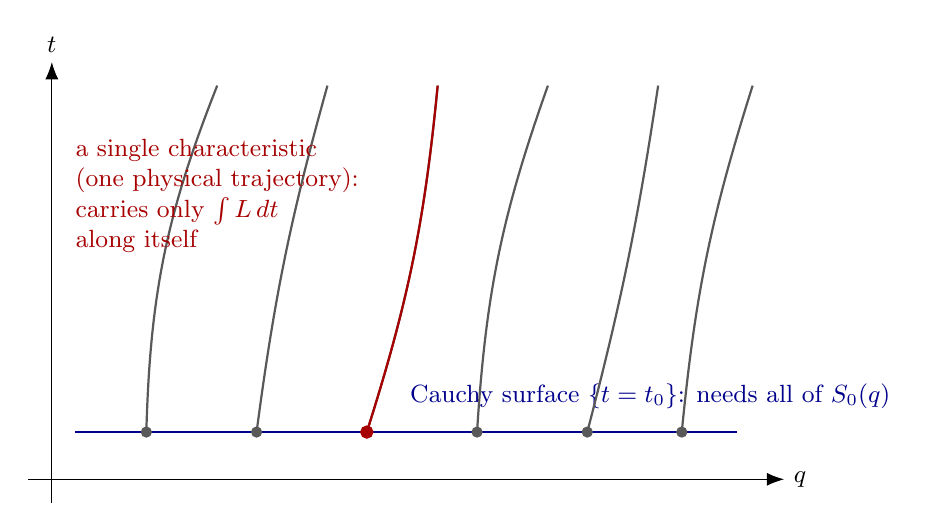
\begin{tikzpicture}[
    surf/.style={thick, blue!55!black},
    char/.style={thick, gray!70!black},
    hero/.style={thick, red!65!black},
    lbl/.style={font=\small}
]
\draw[-{Latex[length=2.2mm]}] (-0.3,0) -- (9.3,0) node[right, font=\small] {$q$};
\draw[-{Latex[length=2.2mm]}] (0,-0.3) -- (0,5.3) node[above, font=\small] {$t$};

\draw[surf] (0.3,0.6) -- (8.7,0.6);
\node[lbl, blue!55!black] at (7.6,1.05) {Cauchy surface $\{t=t_0\}$: needs all of $S_0(q)$};

\foreach \x/\bend in {1.2/10, 2.6/4, 4.0/-6, 5.4/8, 6.8/-3, 8.0/6} {
  \draw[char] (\x,0.6) to[bend left=\bend] (\x+0.9,5.0);
  \filldraw[char] (\x,0.6) circle (1.6pt);
}

\draw[hero] (4.0,0.6) to[bend left=-6] (4.9,5.0);
\filldraw[hero] (4.0,0.6) circle (2pt);
\node[lbl, red!65!black, align=left] at (2.1,3.6) {a single characteristic\\(one physical trajectory):\\carries only $\int L\,dt$\\along itself};

\end{tikzpicture}
\caption{The type mismatch. Cauchy data for~\eqref{eq:HJ} is a whole function $S_0(q)$ needed along the entire horizontal surface $\{t=t_0\}$ (blue), which launches an entire family of characteristics (gray)---one for every $q$, all evolving under Hamilton's equations. A single trajectory (red) is only one of these characteristics: the value of $S$ it carries is already forced to equal $\int L\,dt$, and it says nothing about the surface it was launched from.}
\label{fig:surface-vs-curve}
\end{figure}

\section{What does work, and why it is a different kind of problem}
\label{sec:cauchy}

The correct notion of initial data for~\eqref{eq:HJ} follows directly from Section~\ref{sec:characteristics}: choose the hypersurface $\{t=t_0\}$, which is noncharacteristic everywhere, since the characteristic direction always has $\dot t=1\neq0$ by~\eqref{eq:hj-char} and so is never tangent to a constant-$t$ slice. Data on this hypersurface is simply a function $S_0:Q\to\R$, and the method of characteristics of Section~\ref{sec:characteristics}---run forward from every point of $Q$ at once, not from one point---produces a solution $S(q,t)$ for $t$ near $t_0$, agreeing with $S_0$ at $t=t_0$ \citep{evans2010}.

This is a genuine, well-posed initial-value problem in the only sense available to a PDE: Cauchy data on a noncharacteristic hypersurface, matching data and unknown as the same kind of object (a function of $q$) exactly as Section~\ref{sec:ham-ivp} matched data and unknown for~\eqref{eq:Ham} as the same kind of object (a point of $T^*Q$). It is emphatically not point data, and emphatically not data along one trajectory; Proposition~\ref{prop:trajectory-characteristic} already rules those out.

It is also, even granting the correct kind of data, not a problem that remains well posed for all time. Differentiating the initial momentum field $p_0=\partial S_0/\partial q$ singles out a Lagrangian submanifold $\Lambda_0=\{(q,p_0(q)):q\in Q\}\subset T^*Q$---an $n$-dimensional submanifold on which the canonical one-form $p\,dq$ restricts to the exact form $dS_0$. Flowing every point of $\Lambda_0$ forward under~\eqref{eq:Ham} produces a family of Lagrangian submanifolds $\Lambda_t$, and $S(q,t)$ is recovered from $\Lambda_t$ by integrating the action along each flowed trajectory, exactly as in Section~\ref{sec:counterexample}, for as long as $\Lambda_t$ remains a \emph{graph} over $Q$---that is, for as long as the projection $\Lambda_t\to Q$ stays a diffeomorphism. Where two nearby trajectories launched from $\Lambda_0$ first cross---a \emph{conjugate point}, in the language of the calculus of variations---this projection degenerates, $\Lambda_t$ folds over itself, and $S(q,t)$ ceases to be single-valued: a caustic \citep{arnold1989,gray2009}. So even the correctly posed Hamilton--Jacobi initial-value problem is, in general, only locally well posed in time, for reasons independent of everything in this paper so far and detailed elsewhere \citep{gray2009}.

What matters for the present argument is the contrast in kind between $\Lambda_0$ and a single initial condition $(q_0,p_0)$ for~\eqref{eq:Ham}. The datum $(q_0,p_0)$ is one point of $T^*Q$ and determines one trajectory. The datum $S_0$ is equivalent to an entire $n$-dimensional Lagrangian submanifold $\Lambda_0$---informationally, a continuum of initial conditions $(q,p_0(q))$, one for every $q\in Q$, launched simultaneously. Solving the Hamilton--Jacobi initial-value problem is not solving one instance of Hamilton's initial-value problem; it is solving all of them at once, for a coherent (Lagrangian) family of starting momenta, and then bookkeeping the accumulated action across the whole family. This is why the two ``initial-value problems,'' despite the suggestive parallel in how~\eqref{eq:Ham} and~\eqref{eq:HJ} are written down, are not variations on a theme: one is the initial-value problem for a single particle, the other is the initial-value problem for an entire congruence of particles, and only the second is available to the field $S(q,t)$ that~\eqref{eq:HJ} actually governs.

\section{Why the confusion is natural, and a practice that resembles it}
\label{sec:discussion}

The temptation this paper argues against is not a beginner's mistake so much as an artifact of two genuine features of Hamilton--Jacobi theory that are easy to elide.

First, the equation really is first order in $t$, and really is derived side by side with~\eqref{eq:Ham} in most textbook treatments, inviting the reader to think of $S$ as ``the same kind of thing, evolving the same kind of way'' as $(q,p)$. Section~\ref{sec:two-objects}'s distinction between $\sigma$ and $S$ is easy to lose sight of once both are called ``the action.''

Second, standard practice for actually solving~\eqref{eq:HJ} by separation of variables does involve fixing finitely many constants, and this is often described loosely, in a way that echoes ``initial conditions.'' Jacobi's theorem produces solutions in the form of a \emph{complete integral} $S(q,t;\alpha)$, an $n$-parameter family of solutions of~\eqref{eq:HJ} with $\det(\partial^2S/\partial q\,\partial\alpha)\neq0$; picking out one member of this family by fixing the constants $\alpha$, and further fixing an additive constant $\beta$ via $\partial S/\partial\alpha=\beta$, is exactly the kind of finite-dimensional choice that feels like specifying initial data. But this is a fundamentally different operation from posing a Cauchy problem for the general nonlinear equation~\eqref{eq:HJ}: it selects one member of a family that is \emph{already assumed to solve the PDE for every value of $\alpha$}, rather than constructing a solution from raw data on a hypersurface. The constants $(\alpha,\beta)$ are coordinates on the (typically low-dimensional) solution space one has already found by an ansatz, not Cauchy data for the equation in general. Both practices are legitimate; only one of them is an initial-value problem for a PDE, and it is not the one that resembles fixing a point.

\section{Conclusion}
\label{sec:conclusion}

Hamilton's canonical equations and the Hamilton--Jacobi equation are equivalent formulations of classical mechanics in the precise sense of Jacobi's theorem, but they are not the same kind of equation, and the notion of ``initial data'' that makes one of them well posed does not transfer to the other by analogy. The unknown in Hamilton's equations is a point of a finite-dimensional space, and a point of data at one instant determines it for all time. The unknown in the Hamilton--Jacobi equation is a function on configuration space, and nothing short of an entire function's worth of data on a hypersurface will do---not a point, and, as Proposition~\ref{prop:trajectory-characteristic} shows, not even an entire trajectory's worth of values, because a trajectory is exactly a characteristic curve of the equation, and data along a characteristic is never free data for a first-order PDE. The correctly posed problem exists, is well understood, and is only locally solvable in time for reasons of its own; but it answers a different question from the one Hamilton's initial-value problem answers, computing the action across an entire congruence of trajectories rather than following one. The resemblance between~\eqref{eq:Ham} and~\eqref{eq:HJ} that motivates the search for a pointwise initial-value problem is real, but it is a resemblance in bookkeeping, not in the kind of mathematical object either equation is fundamentally about.

\bibliographystyle{plainnat}
\begin{thebibliography}{9}

\bibitem[Abraham and Marsden(1978)]{abrahammarsden}
Abraham, R. and Marsden, J.~E. (1978).
\textit{Foundations of Mechanics}, 2nd edition.
Benjamin/Cummings, Reading, MA.

\bibitem[Arnold(1989)]{arnold1989}
Arnold, V.~I. (1989).
\textit{Mathematical Methods of Classical Mechanics}, 2nd edition.
Springer, New York.

\bibitem[Courant and Hilbert(1962)]{courant-hilbert1962}
Courant, R. and Hilbert, D. (1962).
\textit{Methods of Mathematical Physics, Volume II: Partial Differential Equations}.
Interscience Publishers, New York.

\bibitem[Evans(2010)]{evans2010}
Evans, L.~C. (2010).
\textit{Partial Differential Equations}, 2nd edition.
Graduate Studies in Mathematics, vol.~19. American Mathematical Society, Providence, RI.

\bibitem[Gray(2009)]{gray2009}
Gray, C.~G. (2009).
Principle of least action.
\textit{Scholarpedia}, 4(12):8291.

\end{thebibliography}

\end{document}
